%!TEX root = Manuscrit.tex
\chapter{Introduction}
\label{chap:intro}
	\citationChap{}{}
	\minitoc
	\newpage


% Début du chapitre
\section{Problématique}

\begin{figure}[t]
	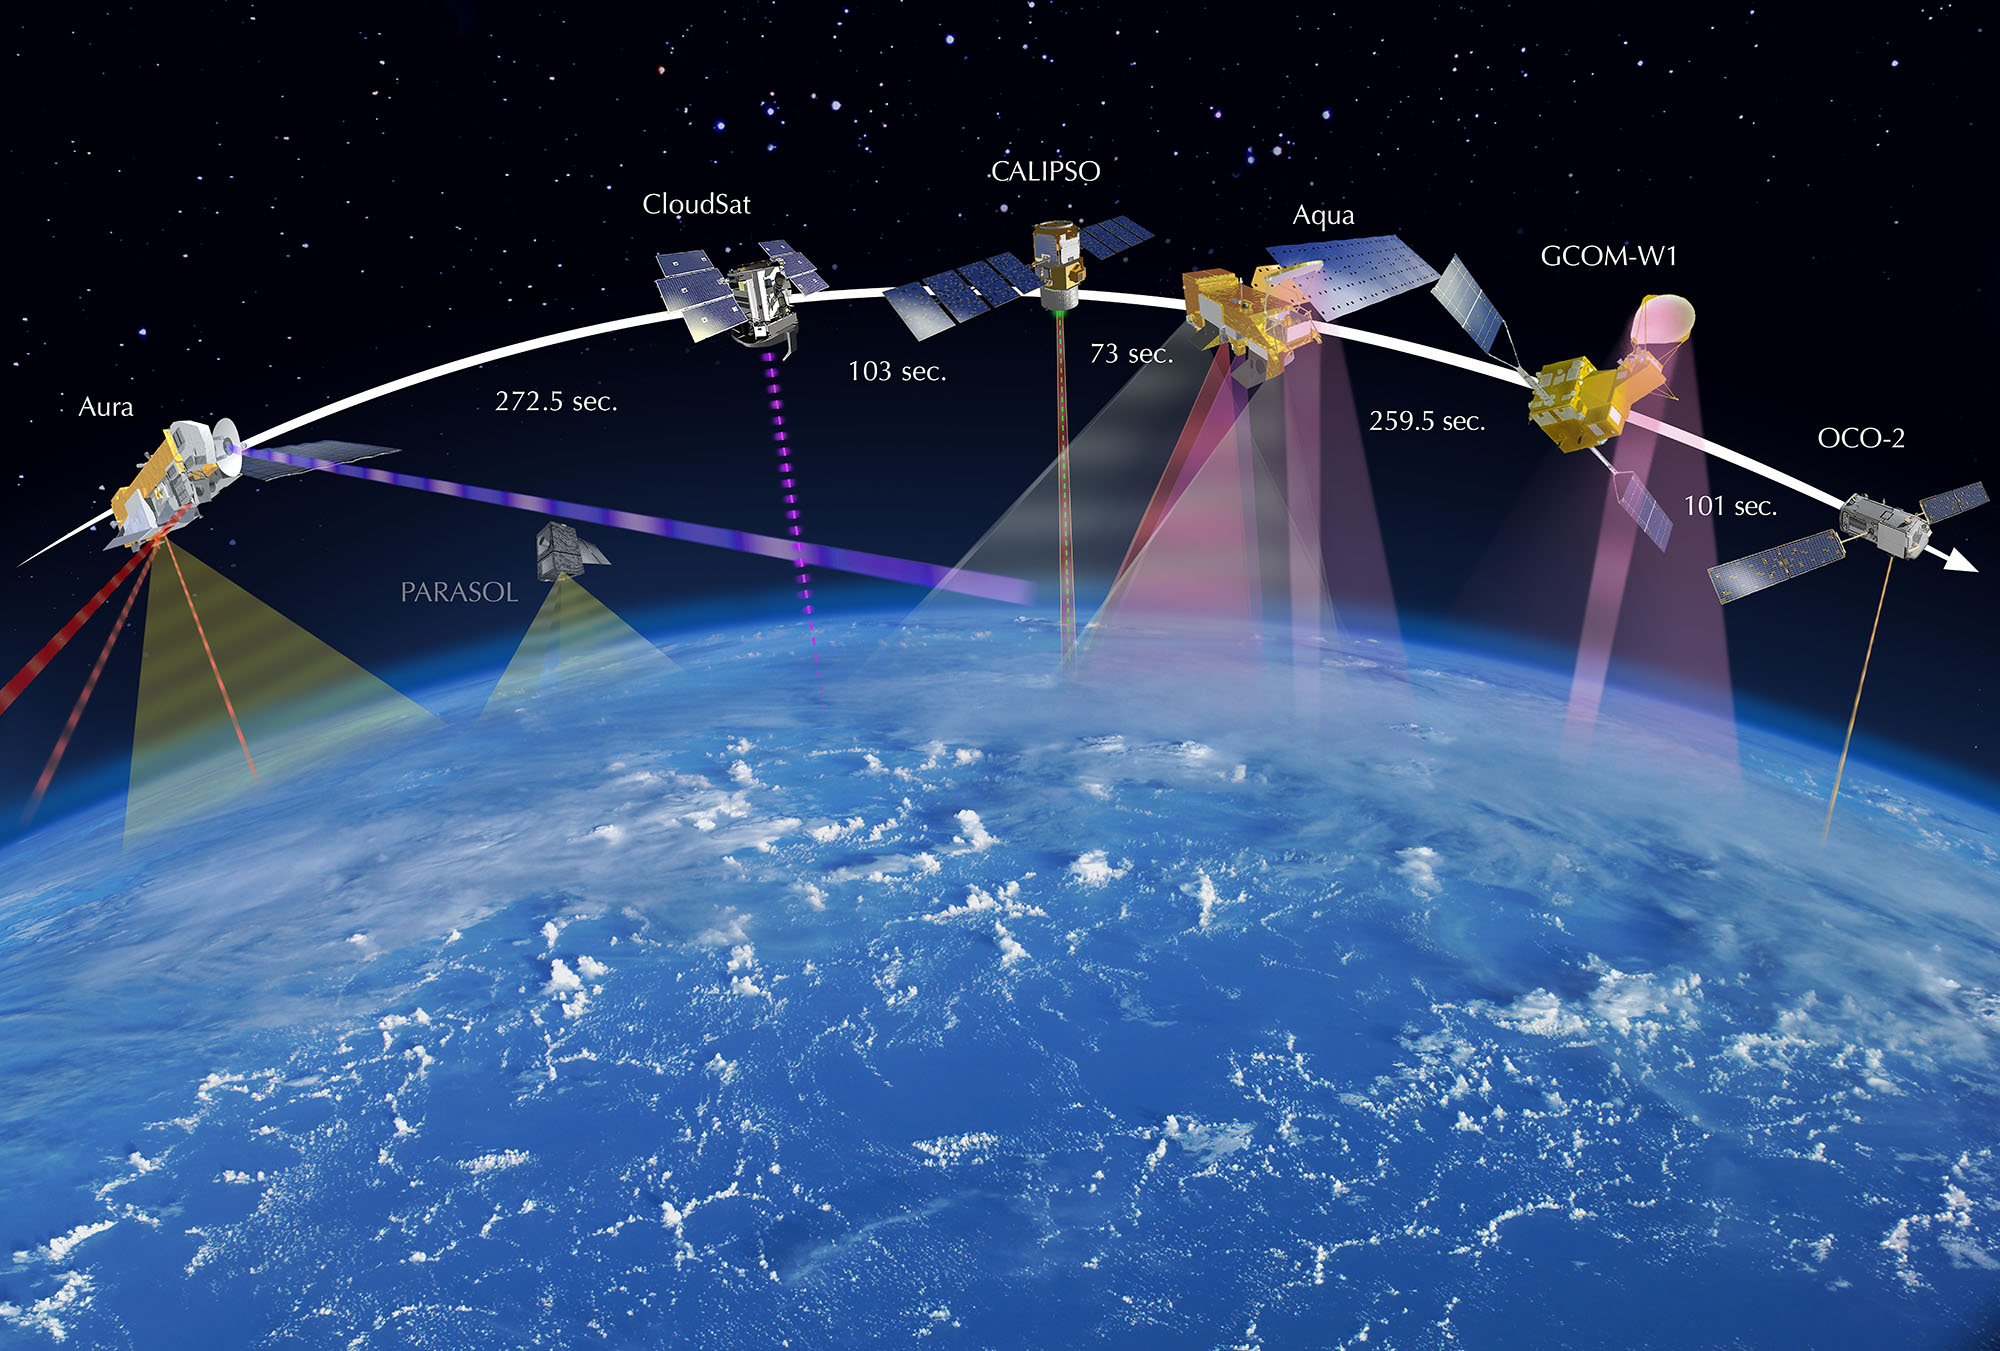
\includegraphics[width=\textwidth]{atrain}
	\caption{Satellites de la constellation A-Train pour l'observation de la Terre en 2018.}
	{\small Crédits image\,: \href{https://commons.wikimedia.org/w/index.php?curid=33645603}{NASA JPL (domaine public)}}
	\label{fig:atrain}
\end{figure}

L'observation est à la base de la méthode scientifique. Tout objet d'étude est susceptible d'être examiné sous toutes ses coutures pour en comprendre les propriétés. La Terre ne fait pas exception à cette logique. Ce n'est donc pas une surprise si, lors de l'avènement des premiers programmes spatiaux, les premiers satellites mis en orbite étaient résolument tournés vers notre planète. En effet, l'altitude a permis à la communauté scientifique d'acquérir une toute nouvelle perspective.

L'imagerie aérienne et satellitaire est donc devenu un outil particulièrement présent dans les sciences modernes. Comprendre la Terre est un enjeu scientifique majeur, et l'observation est le premier pas nécessaire à toute tentative de modélisation. Qu'il s'agisse de météorologie, d'océanographie, d'écologie ou de géographie, les images aéroportées et satellitaires fournissent une information formidablement riche.

L'intensification des efforts pour imager la Terre dans son intégralité à haute fréquence n'a donc rien d'étonnant. Des initiatives telles que \gls{Landsat}, \gls{Sentinel} ou \gls{SPOT} permettent d'imager le globe tout entier chaque semaine. Pour autant, exploiter cette masse de données n'est pas chose aisée. Interpréter et comprendre une image satellite nécessite une expertise forte, aussi bien liée au capteur utilisé pour acquérir l'image qu'aux connaissances relevant du champ d'application visé.

Extraire de l'information de ces images a un intérêt important dans de nombreux domaines applicatifs :
\begin{itemize}
	\item \textbf{Législation} : étude du respect des législations en vigueur concernant les cycles agricoles, surveillance de l'apparition de bâti non autorisé, détection de navires de contrebande\dots
	\item \textbf{Écologie} : suivi de la santé des espaces forêstiers (déforestation, pollution), détection de dégazage pétroliers, suivi des icebergs et évaluation de la fonte des glaces\dots
	\item \textbf{Urbanisme} : étude de la densification du tissu urbain, suivi du maillage routier et ferré\dots
	\item \textbf{Météorologie} : suivi des phénomènes météorologiques intenses (tempêtes, cyclones), étude du réchauffement climatique\dots
\end{itemize}

Ainsi, malgré leur nombre, les photo-interprètes ne peuvent assumer seuls cette responsabilité. L'automatisation présente alors une alternative intéressante. Conférer aux machines la capacité d'interpréter les images de la Terre permettrait de multiplier les observations, pour en tirer à la fois informations et modèles.

C'est le sujet de cette thèse.

Nous cherchons à concevoir, implémenter et de valider des modèles de réseaux de neurones artificiels profonds pour l'interprétation automatisée d'images aériennes et satellites, issues de capteurs multiples, sur une large variété de scènes et pour différents champs d'application.

\begin{figure}[t]
    \centering
    \def\svgwidth{\columnwidth}
    \input{Chapitre1/dessin.pdf_tex}
\end{figure}

\section{Domaine}

Cette thèse se place à l'intersection de trois domaines scientifiques\,: la télédétection, la vision artificielle et l'apprentissage statistique. La litérature en vision par ordinateur est abondante concernant l'interprétation de scènes visuelles et les données de télédétection n'y font pas exception. Récemment, les méthodes dites d'apprentissage profond ont permis de réaliser des avancées considérables en interprétation automatique d'images. Toutefois, l'essentiel de la communauté s'intéresse aux tâches perceptuelles liées à des scènes de la vie quotidienne. En particulier, les applications s'inscrivent souvent dans le cadre d'extraction d'information dans des images ou vdéos multimédias ou à finalité de perception pour un agent robotique autonome. Dans notre cas, les images de télédétection possèdent des propriétés particulières, aussi bien par la physique des capteurs mis en jeu que par les propriétés géométriques des objets étudiés.

\subsection{Images de télédétection}

Les images de télédétection regroupent une grande variété de données acquises par des moyens spatiaux ou aéroportés. Dans une majorité des cas, l'observation se fait au nadir, c'est-à-dire à la verticale du sol. Les capteurs utilisés peuvent aussi bien être actifs que passifs.

Dans tous les cas, les capteurs vont mesurer l'énergie radiative émise par la scène observée. Dans le cas des capteurs actifs, comme le radar ou le lidar, une onde électromagnétique est envoyée et la mesure porte sur celle renvoyée en retour par la scène. Dans le cas des capteurs passifs, l'énergie mesurée pourra soit être l'énergie radiative émise par la scène (capteurs thermiques dans l'infrarouge), soit l'énergie solaire réfléchie (capteurs multispectraux).

En dépit des spécificités des capteurs, plus nombreux et plus variés que les appareils photos et caméras grand publics, le traitement des images de télédétection est proche de celui des images multimédia classiques. En effet, dans les deux cas, il s'agit d'extraire de l'information d'images, une tâche de perception artificielle communément appelée vision par ordinateur. Une communauté existe ainsi à la lisière entre télédétection et vision artificielle, concevant ou adaptant des algorithmes de traitement d'images pour l'observation de la Terre.

\subsection{Apprentissage statistique}

La sémantisation des images d'observation de la Terre passe nécessairement par une étape automatisée. En effet, le volume de données acquises chaque année par les capteurs aéroportés et spatiaux est simplement trop conséquent pour que des photointerprètes humains soient en mesure de les traiter en temps réel.

L'apprentissage statistique permet de déporter l'extraction de connaissances à une machine afin de l'automatiser. Dans la majorité des cas, il s'agit d'estimer la valeur d'un paramètre ou de prendre une décision parmi un éventail de choix. On parle dans le premier cas de régression et dans le second de classification.

Dans le cas de la photointerprétation, l'expert humain réalise une étude des images de télédétection à sa disposition pour en réaliser une cartographie. Il s'agit d'un processus de décision, durant lequel le photointerprète cherche des indices permettant de déclarer qu'un objet ou une région observée appartient à une catégorie précise. L'apprentissage statistique consiste donc à modéliser numériquement ce processus de classification afin de l'automatiser.

Cette modélisation passe par une phase d'apprentissage ou d'entraînement, durant laquelle le modèle est exposé à des exemples, qui viennent alimenter sa base de connaissances. Une fois l'apprentissage terminé, le modèle statistique est alors en mesure de généraliser les décisions prises sur ces exemples à de nouvelles données inédites. La qualité de cette généralisation est le point critique de cette démarche. Une généralisation faible traduit soit un surapprentissage, soit une mauvaise estimation. Dans le premier cas le modèle a pris en compte des biais spécifiques au jeu de données d'entraînement. Dans le second, le modèle est sous-paramétré et n'a pas les données ou les paramètres ne sont pas suffisamment nombreux pour correctement approximer le processus de décision.

L'émergence de l'apprentissage profond dans les années 2000 a fortement contribué à renouveler la littérature en apprentissage statistique. En particulier, les réseaux de neurones profonds, bien que théorisés et mis en application dès les années 1960, ont trouvé une résonance particulière avec l'ère de la donnée massive. Les grandes bases de données d'apprentissage, combinées avec des modèles de réseaux de neurones artificiels profonds et des implémentations parallèle permettant de rendre les calcul traitables en temps raisonnable, ont permis d'importantes avancées en perception artificielle. Le traitement d'images a notamment largement bénéficié de cette conjonction. Dès 2012, les réseaux de neurones convolutifs profonds se sont imposés comme le nouvel état de l'art pour la classification d'images et ont petit à petit conquis une grande partie des tâches de perception visuelle.

Cette thèse se pose ainsi à l'interface entre la télédétection, la vision par ordinateur et l'apprentissage automatique. En particulier, nous nous proposons de mettre en \oe{}uvre des méthodes d'apprentissage profond pour l'interprétation automatique d'images d'observation de la Terre.

\subsection{Vision par ordinateur}

\section{Contributions}

Cette thèse a 4 contributions majeures.
\begin{enumerate}
  \item Elle participe à établir les réseaux de neurones convolutifs comme nouvel état de l'art pour la cartographie automatisée d'images de télédétection.
  \item Elle démontre la possibilité d'étendre les domaines d'application desdits réseaux à l'ensemble des capteurs optiques usuels.
  \item Elle montre qu'il est possible et pertinent d'utiliser les informatoins présentes dans plusieurs capteurs lorsque c'est possible.
  \item Elle montre que ces approches ne se confinent pas à des cas spécifiques, mais peuvent s'étendre à l'ensemble du globe.
\end{enumerate}

%\bibliographystyle{francaissc}
%\bibliography{Chapitre1/Biblio}
